The version of PMCLP where the facilities are ellipses that can be freely rotated was first introduced in \cite{andreta} where an exact and a heuristic method were developed for it. In comparison with MCE, this problem introduces a new variable that is responsible for determining the angle of rotation of every ellipse, making MCER a more challenging problem. We propose an algorithm for MCER which is able to obtain optimal solutions for every instance proposed in \cite{andreta} including the ones its exact method could not, and its heuristic obtained non-optimal ones.

\begin{definition}
	Two solutions $Q$ and $Q'$ of MCER, are said to be equivalent to each other if \mbox{$\cup_{j=1}^m \Pp \cap E_j(q_j, \theta_j) = \cup_{j=1}^m \Pp \cap E_j(q_j', \theta_j')$}. Also, if $\cup_{j=1}^m \Pp \cap E_j(q_j, \theta_j) \subset \cup_{j=1}^m \Pp \cap E_j(q_j', \theta_j')$, then we say that $Q' \succ Q$.
\end{definition}

%\begin{definition}
%	Let $x \in \R^2$, we define $\angle x$ as the angle between the vector $(1, 0)$ and $x$.
%\end{definition}

Next, we introduce a lemma which states that any optimal solution of MCER has an equivalent solution where every ellipse that covers at least two points has two points on its border.

\begin{lem}\label{lema:mce_2b}
	Let $Q^*$ be a solution of MCER for an instance $(\Pp, \Ww, \{(a,b)\})$.
	If $|\Pp \cap E(q^*, \theta^*)| \ge 2$, then there exists a solution $Q$ for the same instance, such that $Q \succ Q^*$, and $|\Pp \cap \partial E(q, \theta)|\ge 2$.
\end{lem}

\begin{proof}
	First, let $\theta=\theta^*$ and ignore the angle of rotation as it does not change, and assume that we are dealing with an axis-parallel ellipse.
	
	Let $A=\Pp \cap E(q^*, \theta^*)$ and $X=\cap_{p \in A}E(p, \theta^*)$ be the region of intersection of ellipses centered at each point in $A$. By \cite{bi}, the vertices of $\partial X$ are in the set of pairwise intersections of $\{\partial E(p, \theta^*)\colon p \in A\}$. Setting $q$ as any of these vertices makes $E(q, \theta)$ have two points on its border.	
\end{proof}

%Next, we define, for an optimal solution, a set of equivalent solutions, such that any ellipse covering more than one point contains at least two points.

%\begin{definition}
%	Let $Q^*$ be an optimal solution of MCER. We define $\Pi(Q^*)$ as the set of every equivalent solution to $Q^*$, such that for any $Q \in\Pi(Q^*)$, for $j\in\{1, \dots, m\}$ with $|\Pp \cap E_j(q_j^*, \theta_j^*)|\ge2$, we have $|\Pp \cap \partial E_j(q_j', \theta_j')| \ge 2$.
%\end{definition}

Next, we introduce a notation that helps us characterize angles which given an ellipse rotated by it and two points, it is possible to find a center for the ellipse, such that it contains both points.

\begin{definition}\label{def:feasible_angle}
	Let $E$ be the coverage region of an ellipse and $u, v \in \R^2$. An angle $\theta \in [0, \pi)$ is said to be $(E, u, v)$-feasible if there is $q \in \R^2$ such that $\{u, v\} \subset \partial E(q, \theta)$.
	In addition to that, the set of $(E, u, v)$-feasible angles is referred to as 
	
	\begin{equation}
	\Phi(u, v) := \{\theta \in [0, \pi) : \theta \textnormal{ is a } (E,u,v)\textnormal{-feasible angle}\}.
	\end{equation}
	%We also define $\tilde{\Phi}_j(u,v)$ as the angle which makes $E_j$'s major-axis be parallel to the line that passes through $u$ and $v$. Note that if $\Phi_j(u,v) \neq \emptyset$, then $\tilde{\Phi}_j(u,v) \in \Phi_j(u,v)$ as the longest segment that crosses an ellipse is its major-axis.
\end{definition}

\begin{figure}[H]
	\centering
	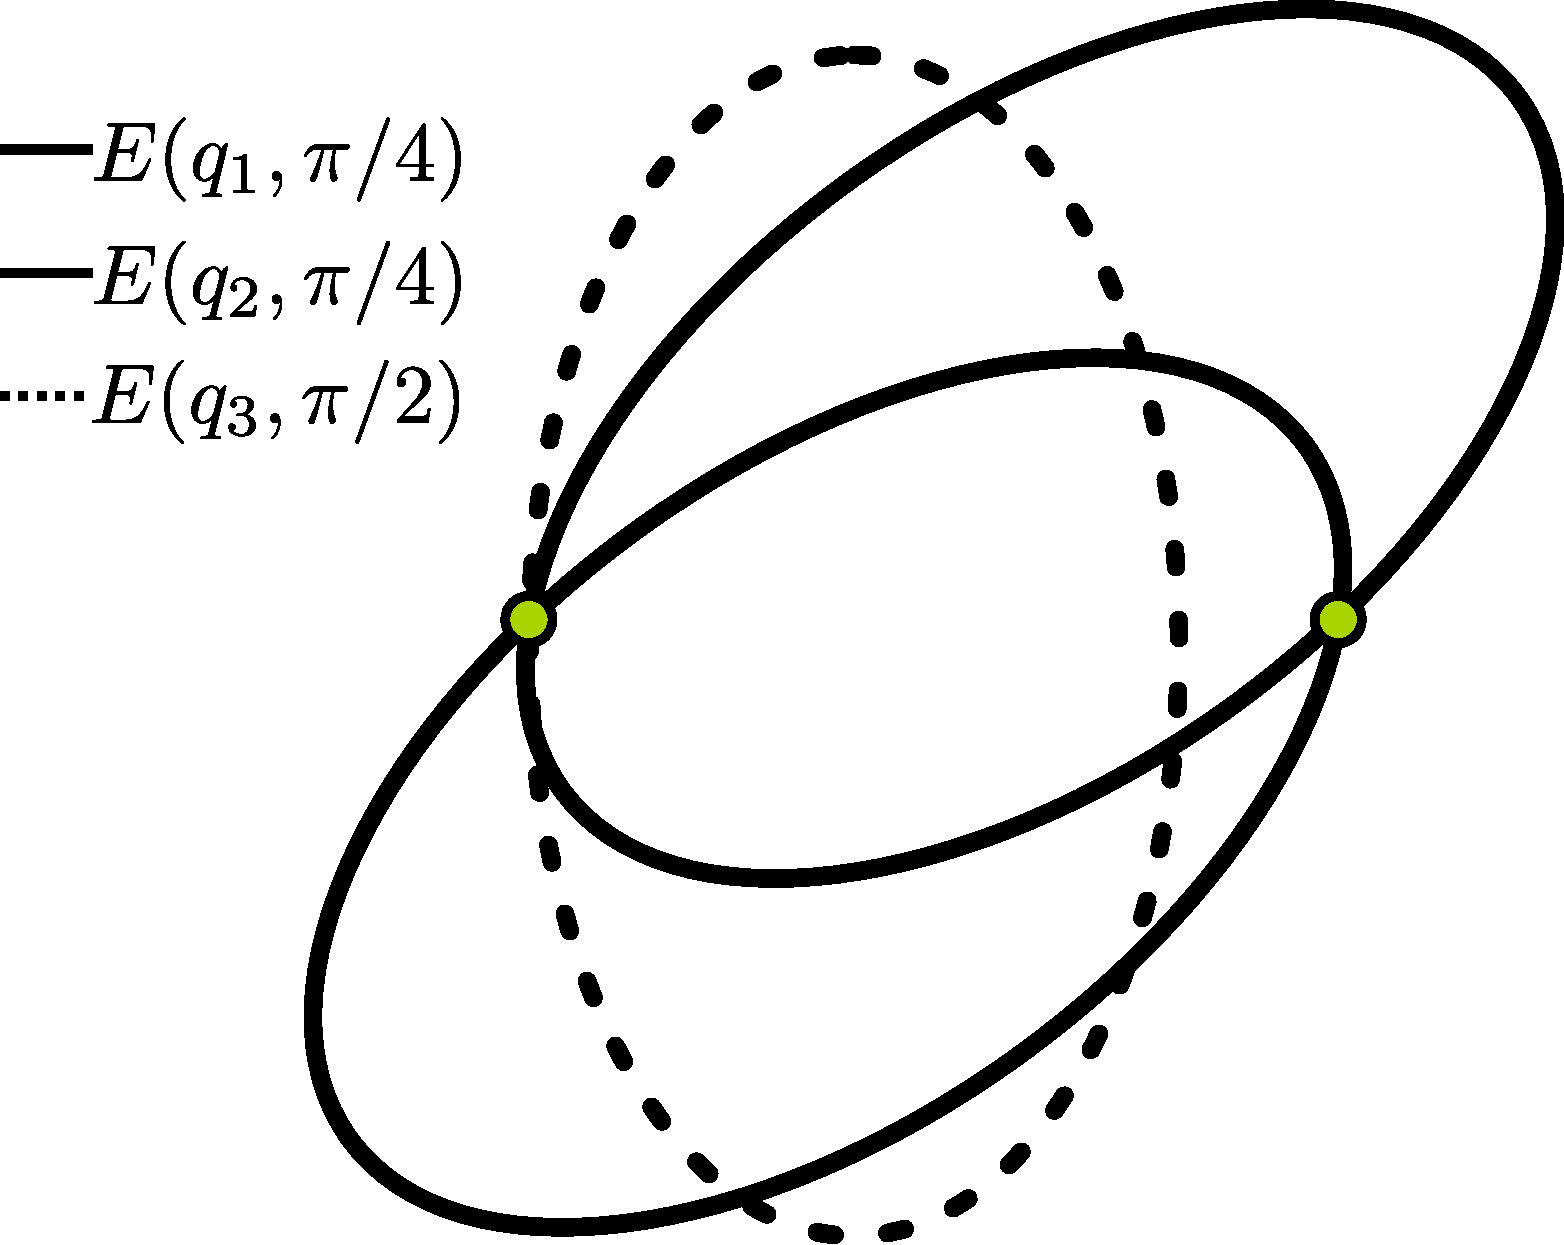
\includegraphics[scale=.22]{figures/feasible-angle2}
	\caption{A $(E, u, v)$-feasible angle and a not $(E, u, v)$-feasible angle.}
	\label{fig:feasible-angle}
\end{figure}


Next we open a parenthesis to discuss the problem of deciding when it is possible to fit two points on an ellipse.

\begin{lem}\label{lema:l-function}
	Given an instance $(\Pp, \Ww, \{(a, b)\})$ of MCER, if $u, v \in \Pp$ have the same $y$-coordinate and $||u-v||_2 \le 2a$, then $\Phi(u,v) = [0, \alpha] \cup [\pi - \alpha, \pi)$, for some $\alpha \in [0, \pi/2]$.
\end{lem}

\begin{proof}
	
	Consider an axis-parallel ellipse with shape parameters $(a, b)\in\R^2_{>0}$, centered at the origin, and a line represented by the equation $y=mx+c$, with $m, c\in \R$. Suppose that this line intersects the ellipse at least at one point. By plugging the line's equation into $x^2/a^2+y^2/b^2=1$, it is possible to obtain the distance between the intersection points. The final expression is given by
	\begin{equation*}\label{eq:dist_line_ellipse}
	D(m, c)=\dfrac{\sqrt{(a^2m^2+b^2-c^2)(4a^2b^2(1+m^2))}}{(a^2m^2+b^2)},
	\end{equation*}
	with $D : \R^2 \mapsto \R_{\ge0}$ being a function of the line parameters $(m, c)$.
	If $D(m, c) = ||u-v||_2$, then there exists $q_1, q_2 \in \R^2$, such that $\{u, v\} \subset \partial E(q_1, \tan{m})$ and $\{u, v\} \subset \partial E(q_2, \pi-\tan{m})$. It is also possible to see that, when $m$ is fixed, $D(m, c)^2$ is a parabola, and that $D(m, c)$ is maximized at $c=0$.  
	Following that, we define a function $L:\R\mapsto\R$ as
	
	\begin{equation}\label{eq:function-l}
	L(m):= D(m, 0)^2 = \dfrac{(a^2m^2+b^2)(4a^2b^2(1+m^2))}{(a^2m^2+b^2)^2},
	\end{equation}
	which describes the maximum distance between points of an ellipse-line intersection considering all lines with $m$ angular coefficient. From that, if $L(m) \ge ||v-u||_2^2$, then there exists $q_1, q_2\in\R^2$, such that $\{u, v\} \subset \partial E(q_1, \tan{m})$, and $\{u, v\} \subset \partial E(q_2, \pi-\tan{m})$.
	
	It is possible, by calculating the derivatives, to conclude that $L$ has its maximum at $m=0$, is increasing in $[0, \infty)$, is decreasing in $(-\infty, 0]$, and attains every value in the interval $(4b^2, 4a^2]$. Notice that $L$ never hits $4b^2$ because that is the distance between the intersection of the ellipse with a vertical line.
	%In \autoref{fig:L-function-plot}, an example of function $L$ is shown with $(a, b) = (2, 1)$.
	
	If $\inf{L} \ge ||u-v||_2^2$, then $\Phi(u,v) = [0, \pi)$.
	Otherwise, let $\beta \in \R$, $\beta \ge 0$, such that $L(\beta) = ||u-v||_2^2$, then as $m>\beta$, we have $L(m) < ||u-v||_2^2$, which means that it is impossible to make the ellipse contain $u$, and $v$.
	As $L$ is an even function, the same can be said for $m < \beta$. Therefore, we conclude that $\Phi(u,v)=[0, \tan(\beta)] \cup [\pi-\tan(\beta), \pi)$.
\end{proof}
%\begin{figure}[H]
%	\centering
%	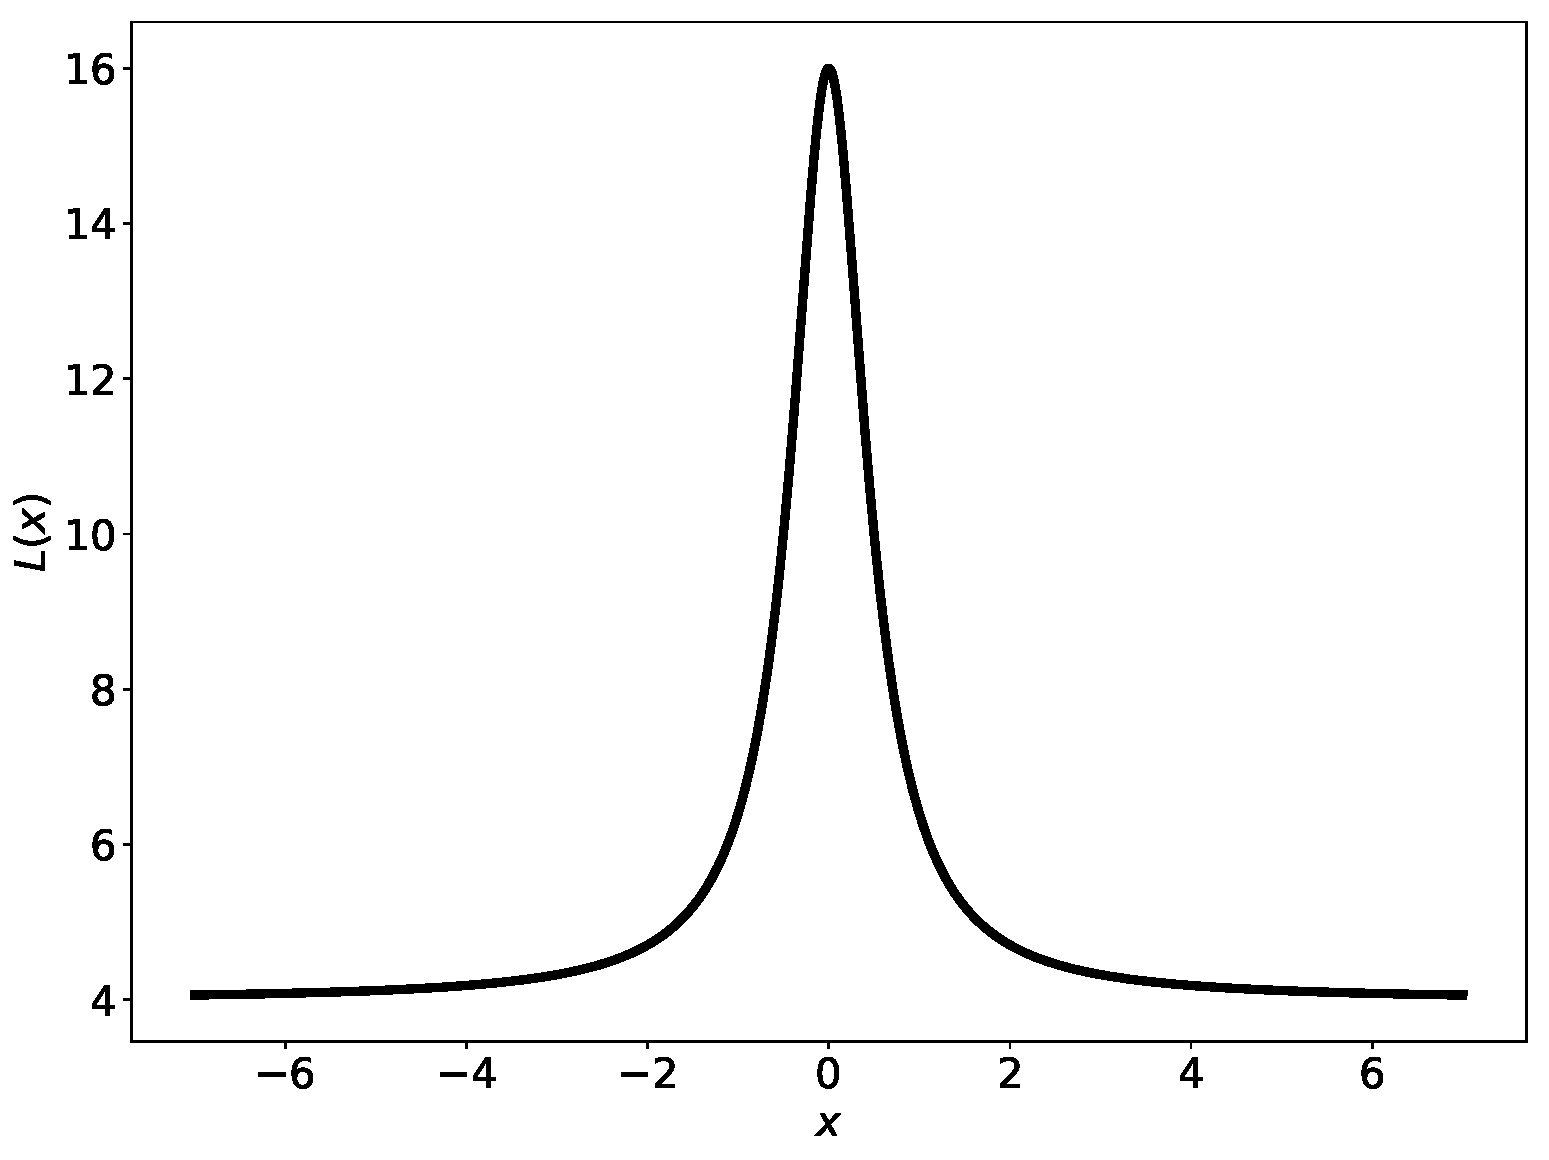
\includegraphics[scale=.4]{../tex/figures/L-function-plot}
%	\caption{Plot of function $L$ in the interval $[-7, 7]$.}
%	\label{fig:L-function-plot}
%\end{figure}



%%% Fim L function


\begin{lem}\label{lema:3pnts}
	Let $Q^*$ be a solution of MCER for the instance $(\Pp, \Ww, \{(a, b)\})$, such that $|\Pp \cap E(q^*, \theta^*)|\ge2$.
	If for all $\bar{Q} \succ Q^*$, $|\Pp \cap \partial E(\bar{q}, \bar{\theta})| < 3$, then there exists $\{u, v\} \subset \Pp \cap E(q^*, \theta^*)$, such that for all $\theta\in \Phi(u,v)$ there exists $q \in \R^2$, such that $(q, \theta)$ is equivalent to $Q^*$.
\end{lem}

\begin{proof}
	According to \autoref{lema:mce_2b}, there exists $\{u, v\} \subset \Pp \cap E(q^*, \theta^*)$, such that $Q' \succ Q^*$ exists, and $\{u, v\} \subset \partial E(q', \theta^*)$. Therefore, $\theta^*\in\Phi(u,v)$.
	
	Suppose that $u$ and $v$ have the same $y$-coordinate, if they do not, a rotation can be applied to make them do. Then, by \autoref{lema:l-function}, $\Phi(u,v)=[0, \alpha] \cup [\pi-\alpha, \pi)$, for some $\alpha \in [0, \pi/2]$. Then, if we rotate the coordinate system by $\pi-\alpha$, we obtain $\Phi(u,v)=[0, 2\alpha]$.
	
	With this result in hand, we can use a continuity argument to complete our proof as follows.
	Let $\delta : \Phi(u,v) \mapsto \R^2$ be a continuous function which takes an angle $\theta\in\Phi(u,v)$ and returns a center, such that $\{u,v\} \subset \partial E(\delta(\theta), \theta)$, and, from solution $Q'$, $\delta(\theta') = q'$. Notice that, in general, for any angle in $\Phi(u,v)$, there are two possible centers that make $\{u,v\} \subset \partial E(\delta(\theta), \theta)$ (see \autoref{fig:feasible-angle} for an example), however, imposing $\delta(\theta') = q'$ makes $\delta$ be a well-defined continuous function. This is shown in \autoref{fig:lema-3-points} where $\delta$ is plotted for the whole interval $\Phi(u,v)$.
	
	Let $w\in \Pp \setminus \{u,v\}$, then we define $f_w  : [0, \pi) \mapsto \R_{\ge0}$ to be a function that takes an angle of rotation $\theta$ and returns the elliptical distance $||\cdot||_{a,b,\theta}$ to the center $\delta(\theta)$; that is $f_w(\theta)=||w-\delta(\theta)||_{a,b,\theta}$.
	We have that if $w \in \Pp \cap E(q^*, \theta^*)$, then $f_w(\theta^*) \le 1$; and if $w \not\in \Pp \cap E(q^*, \theta^*)$, then $f_w(\theta^*) > 1$.
	
	Therefore, if there exists $\theta\in\Phi(u,v)$, such that for all $q\in\R^2$, $(q, \theta)$ is not equivalent to $Q^*$, then there exists either $w \in \Pp \cap E(q^*, \theta^*)$, with $f_w(\theta)>1$, or $w \not\in \Pp \cap E(q^*, \theta^*)$, with $f_w(\theta)\le 1$. Because $f_w$ is continuous, there exists $\bar{\theta}\in\Phi(u,v)$, such that $f_w(\theta)=1$, implying that $|\Pp \cap \partial E(\delta(\bar{\theta}), \bar{\theta})| \ge 3$.
\end{proof}

\begin{figure}[H]
	\centering
	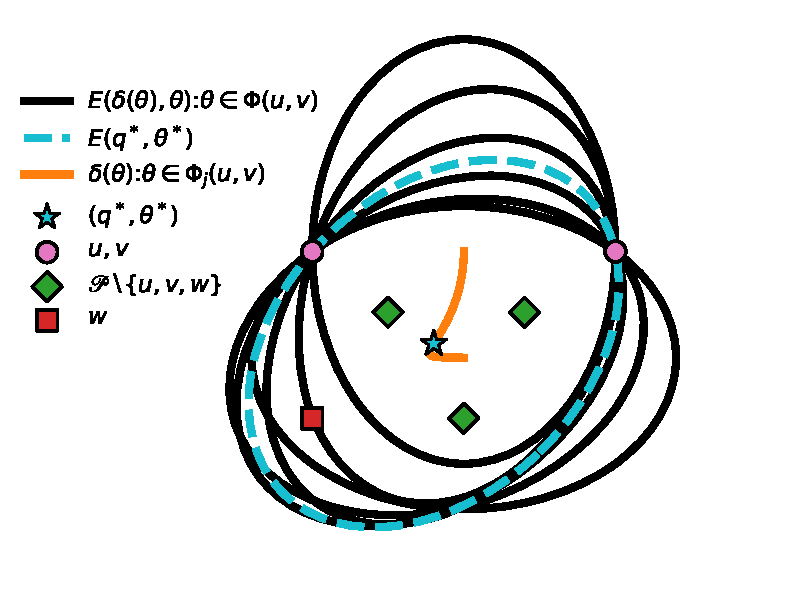
\includegraphics[scale=.7]{figures/lema-3-points}
	\caption{A visualization of \autoref{lema:3pnts}.}
	\label{fig:lema-3-points}
\end{figure}